\section*{Ejercicio \#2}
Como paso siguiente procedemos a implementar los algoritmos de ordenamiento a continuación:
\begin{itemize}
    \item \href{https://github.com/syordya/CSUNSA-EDA/tree/master/Practica01/code/BubbleSort}{\textbf{Bubble Sort}}: Complejidad $O(n^2)$.\\
    Es  un  algoritmo  de  ordenamiento  muy  sencillo  que  funciona  revisando  cada elemento de la lista que se está ordenando e intercambiándolo con otra posición, de tal manera que el más grande o pequeño según sea el orden va subiendo, de ahí su nombre.\cite{marisolanalisis}
    \item \href{https://github.com/syordya/CSUNSA-EDA/tree/master/Practica01/code/CountingSort}{\textbf{Counting sort}}: Complejidad $O(n+k)$
    Counting sort es una técnica de ordenamiento basada en \textit{llaves} dentro de un rango en específico.
    \item \href{https://github.com/syordya/CSUNSA-EDA/tree/master/Practica01/code/HeapSort}{\textbf{Heap sort}} : Complejidad $O(nlogn)$.
    Heap sort usa la estructura de datos conocida como Binary heap. Es similar al algoritmo de selección donde primero encontramos el máximo elemento y lo colocamos al final.
    \item \href{https://github.com/syordya/CSUNSA-EDA/tree/master/Practica01/code/InsertionSort}{\textbf{Insertion sort}} : Complejidad $O(n^2)$.
    Insertion sort divide el array en la parte ordenada y en la que está por ordenar. Los valores de la región desordenada se escogen uno a uno y se colocan en la posición correcta del arreglo ordenado. \cite{cormen}
    \item \href{https://github.com/syordya/CSUNSA-EDA/tree/master/Practica01/code/MergeSort}{\textbf{Merge sort}}: Complejidad $O(n log n)$.
    Merge sort es un algoritmo de divide y conquista. Se divide el arreglo en dos y así sucesivamente. La función \verb!merge()! es usada para unir las dos partes, se asume que los arreglos \(arr[1..m]\) y \(arr[m+1..r]\)  estan ordenados.
    \item \href{https://github.com/syordya/CSUNSA-EDA/tree/master/Practica01/code/QuickSort}{\textbf{Quick sort}}: Complejidad $O(nlogn)$.
    Un algoritmo de divide y conquista en el cual se elige un elemento como pivote y se particiona el arreglo alrededor de este.
    \item \href{https://github.com/syordya/CSUNSA-EDA/tree/master/Practica01/code/SelectionSort}{\textbf{Selection sort}}: Complejidad $O(n^2)$.\\
    Es un algoritmo  de  ordenamiento que  busca el  mínimo elemento  de  la  lista,  lo intercambia con el primero, busca el siguiente mínimo en el resto de la lista y lo intercambia con el segundo, hasta llegar al final de la lista.\cite{marisolanalisis}
\end{itemize}

Para esta tarea usamos los lenguajes \verb!C++!, \verb!Java! y \verb!Python!. Las implementaciones se encuentra en la carpeta \href{https://github.com/syordya/CSUNSA-EDA/tree/master/Practica01/code}{code} del repositorio de la Práctica01.


Para ejecutar los algoritmos en el lenguaje \verb!C++! lo realizamos de la siguiente forma, pasando como entrada, al ejecutable, el archivo \verb!entrada.txt!, el cual contiene los vectores de números aleatorios generados previamente.%Ver figura \ref{fig:ejecucion-cpp}.
\begin{figure}[H]
  \centering
  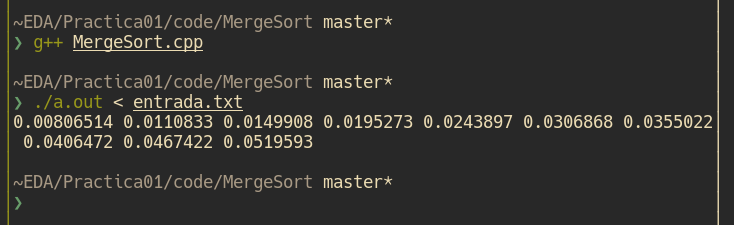
\includegraphics[width=0.8\textwidth]{ejecucion-cpp}
  \label{fig:ejecucion-cpp}
\end{figure}

De la misma forma en \verb!Python!.% Ver figura \ref{fig:ejecucion-python}
\begin{figure}[H]
  \centering
  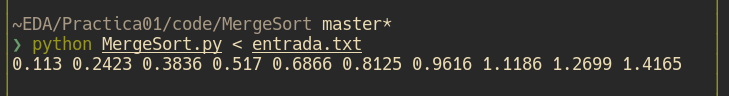
\includegraphics[width=0.8\textwidth]{ejecucion-python}
  \label{fig:ejecucion-python}
\end{figure}

y en \verb!Java!.% Ver figura \ref{fig:ejecucion-java}
\begin{figure}[H]
  \centering
  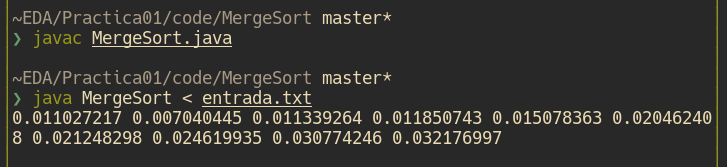
\includegraphics[width=0.8\textwidth]{ejecucion-java}
  \label{fig:ejecucion-java}
\end{figure}

\iffalse
% ---- Para poner dos imágenes (una a lado de otra) ----
Como se muestra en la figuras \ref{fig:act-1_a} y \ref{fig:act-1_b}.

\begin{figure}[H]

\centering

\begin{minipage}{0.75\textwidth}
  \centering
  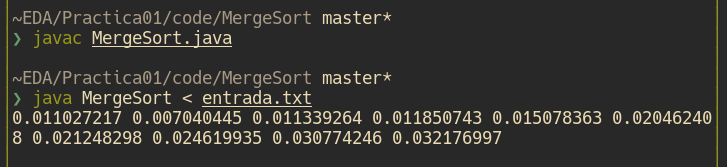
\includegraphics[width=0.8\textwidth]{ejecucion-java}
  \caption{blablablabalbalabla.}
  \label{fig:act-1_a}
\end{minipage}\hfill

\begin{minipage}{0.75\textwidth}
  \centering
  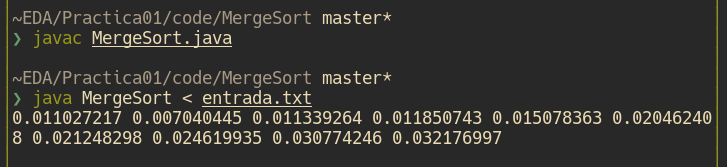
\includegraphics[width=0.8\textwidth]{ejecucion-java}
  \caption{blablablslablala}
  \label{fig:act-1_b}
\end{minipage}

\end{figure}

% ---- Para colocar una imagen ----
Como se muestra en la figura \ref{fig:act-3}
\begin{figure}[H]
  \centering
  \includegraphics[width=0.8\textwidth]{act-3}
  \caption{Tabla de subneteo para la red 192.168.100.0.}
  \label{fig:act-3}
\end{figure}
\fi